\section{Campo elétrico e operações com vetores}

\frame{
	\frametitle{Campo elétrico}
	\begin{block}{Introdução}
		No tópico anterior estudamos a força de interação entre duas partículas eletrizadas. Agora iremos estudar o \textbf{mecanismo dessa força}, estudando o conceito de campo elétrico.
	\end{block}
}

\frame{
	\frametitle{Campo elétrico}
	\begin{block}{Contextualização}
		\begin{itemize}
			\item Os efeitos elétricos que ocorrem nas proximidades de cargas elétricas são associados à existência de um campo elétrico no local; este interage com a \textbf{carga de prova}.
			\item É importante perceber que um campo elétrico só pode ser detectado a partir da interação do mesmo com uma carga de prova, se não existir interação com a carga significa que o campo não existe naquele local.
			\item Um exemplo típico é a interação do cabelo de uma pessoa com a tela de uma televisão convencional, pois as cargas elétricas da televisão interagem com os cabelos, deixando-os arrepiados.
		\end{itemize}
	\end{block}
}


\frame{
	\frametitle{Campo elétrico}
	\begin{block}{Motivação}
		Assim como o nosso planeta possui um campo gravitacional, uma carga elétrica $Q$ também tem um campo que pode influenciar as cargas de prova $q$ nele colocadas.
		
		\begin{itemize}
			\item Campo gravitacional: $g = \dfrac{P}{m}$
			\item Campo elétrico: $E = \dfrac{F}{q}$
		\end{itemize}
	\end{block}
}

\frame{
	\frametitle{Campo elétrico}
	\begin{block}{Definição}
		$$E = \dfrac{F}{q}$$
		A intensidade do campo elétrico ($E$) é definido como o quociente entre as forças de interação ($F$) das cargas geradoras do campo ($Q$) e de prova ($q$) e da própria carga de prova ($q$).
		$$E = \dfrac{F}{q} = \dfrac{K \ \dfrac{Q \ q}{d^2}}{q} \implies \boxed{E = K \ \dfrac{Q}{d^2}}$$
		\begin{itemize}
			\item A unidade de campo elétrico é \si{\newton\per\coulomb}.
		\end{itemize}
	\end{block}
}

\frame{
	\frametitle{Campo elétrico}
	\begin{block}{Terminologias}
		\begin{itemize}
			\item Chama-se \textbf{campo elétrico} o campo estabelecido em todos os pontos do espaço sob a influência de uma carga geradora de intensidade $Q$, de forma que qualquer carga de prova de intensidade $q$ fica sujeita a uma força de interação (atração ou repulsão) exercida por $Q$.
			\item Já uma \textbf{carga de prova}, para os fins que nos interessam, é definida como um corpo pontual de carga elétrica conhecida, utilizado para detectar a existência de um campo elétrico, também possibilitando o cálculo de sua intensidade.
		\end{itemize}
	\end{block}
}

\frame{
	\frametitle{Campo elétrico}
	
	\centering
	
	\setmyunit{0.25cm}
	\begin{tikzpicture}
		\draw (0,0) circle (2) node {$ Q $};
		
		\foreach \x in {3,4,...,12} {
			\draw[dotted] (0,0) circle (\x);
		}
	\end{tikzpicture}
%	\centerline{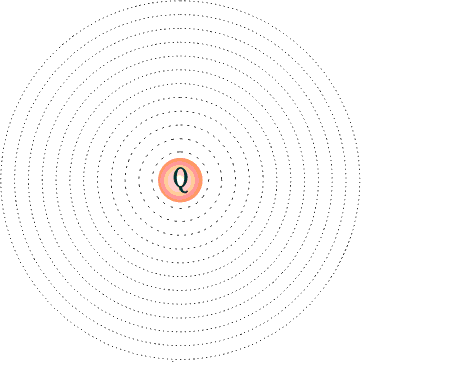
\includegraphics[width=0.7\linewidth]{Figuras/Ch06/campo.png}}
}

\frame{
	\frametitle{Introdução ao vetor campo elétrico}
	\begin{block}{Definição}
		O campo elétrico $\vec{E}$ é uma grandeza vetorial que existe em cada ponto do espaço. O campo elétrico em um local indica a força que poderia atuar sobre uma carga unitária de teste positiva se colocada naquele local. Podemos definir como a \textbf{força elétrica normalizada}, isto é, a força experimentada por uma carga de teste que tem um valor de $+1$.
	\end{block}
}

\frame{
	\frametitle{Introdução ao vetor campo elétrico}
	\begin{block}{Contextualização}
		Imagine uma pequena carga imaginária de teste positiva colada à extremidade de um bastão imaginário. Certifique-se que o bastão imaginário não conduz, como madeira ou plástico. Explore o campo elétrico mantendo a carga de teste em vários locais. A carga de teste será empurrada ou puxada pela carga circundante. A força que a carga de teste experimenta (valor e direção), dividida pelo valor da pequena carga teste, é o vetor do campo elétrico nesse local. \textbf{Mesmo que você remova a carga de teste, ainda há um campo elétrico no local.}
	\end{block}
}

\frame{
	\frametitle{Operação com vetores}
	\begin{block}{Soma - Lei dos cossenos}
		$$\vec{R}^{\,2} = \vec{a}^{\,2} + \vec{b}^{\,2} - 2 \ \vec{a} \ \vec{b} \ \cos \ \alpha$$
		$$\vec{R}^{\,2} = \vec{a}^{\,2} + \vec{b}^{\,2} - 2 \ \vec{a} \ \vec{b} \ \cos \ (\ang{180}-\theta)$$
		$$\vec{R}^{\,2} = \vec{a}^{\,2} + \vec{b}^{\,2} + 2 \ \vec{a} \ \vec{b} \ \cos \ \theta$$
	\end{block}

	\vspace{0.3cm}
	\setmyunit{1.5cm}

	\begin{minipage}{0.49\linewidth}
		\centering
		
		\begin{tikzpicture}
			\draw[-Latex] 
				(0,0) -- node[below] {$ \vec{b} $} +(2,0) coordinate (bs);
			\draw[-Latex]
				(0,0) -- node[left] {$ \vec{a} $} +(60:2) coordinate (a);
				
			\draw[dashed] (0,0) ++(2,0) -- ++(60:2) coordinate (C);
			\draw[gray] (2,0) -- ++(30pt,0) coordinate (b);
			
			\coordinate (O) at (0,0);
			
			\draw[dashed] (0,0) +(60:2) -- (C);
			
			\draw[-Latex] (0,0) -- node[above] {$ \vec{R} $} (C);
			
			\pic[ang,gray,->, angle eccentricity=1.4,"$ \theta $" {inner sep=1pt, shift={(2pt,-5pt)}}] {angle=b--O--a};
			\pic[ang,gray,->,"$ \theta $"] {angle=b--bs--C};
			
		\end{tikzpicture}
	\end{minipage}
	\hfill
	\begin{minipage}{0.49\linewidth}
		\centering
		
		\begin{tikzpicture}
			\draw[-Latex] (0,0) coordinate (O) -- node[below] {$ \vec{b} $} ++(2,0) coordinate (b);
			\draw[-Latex] (2,0) -- node[right] {$ \vec{a} $} ++(60:2) node[coordinate,name=C] {};
			\draw[-Latex] (0,0) -- node[above] {$ \vec{R} $} (C);
			
			\pic[ang,gray,->,angle eccentricity=1.4,"$ \ang{180}-\theta $" rotate=30] {angle=C--b--O};
		\end{tikzpicture}
	\end{minipage}
}

\frame{
	\frametitle{Operação com vetores}
	\begin{block}{Lei dos senos}
		$$\dfrac{a}{sen \ \alpha} = \dfrac{b}{sen \ \beta} = \dfrac{c}{sen \ \theta}$$
	\end{block}

	\vspace{0.5cm}

	\centering
	\begin{tikzpicture}[scale=1.3]
		\draw (0,0) -- node[below] {$ c $} ++(3,0) -- node[right] {$ a $} ++(140:2) coordinate (C);
		
		\draw (0,0) -- node[left,yshift=2pt] {$ b $} (C);
		
		\coordinate (O) at (0,0);
		\coordinate (B) at (3,0);
		
		\pic[ang, "$ \alpha $"] {angle = B--O--C};
		\pic[ang, "$ \beta $"] {angle = C--B--O};
		\pic[ang, "$ \theta $"] {angle = O--C--B};
	\end{tikzpicture}
	
%	\centerline{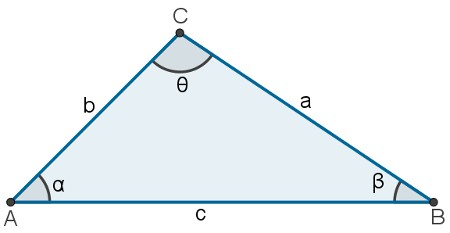
\includegraphics[width=0.7\linewidth]{Figuras/Ch06/leisen.jpg}}
}

\frame{
	\frametitle{Operação com vetores}
	\begin{block}{Decomposição de vetores}
		$$\vec{V_x} = \vec{V} \ \cos \ \alpha$$
		$$\vec{V_y} = \vec{V} \ \sen \ \alpha$$
		$$\tg \ \alpha = \dfrac{\vec{V_y}}{\vec{V_x}}$$
	\end{block}
	
%	\vspace{0.3cm}
	\setmyunit{1.5cm}

	\centering
	\begin{tikzpicture}
		\draw[->] (-0.3,0) -- (2.5,0) node[right] {$ x $} coordinate (x);
		\draw[->] (0,-0.3) -- (0,1.5) node[above] {$ y $} coordinate (y);
		
		\draw[thick, -Latex] (0,0) -- node[left] {$ \vec{V_y} $} (0,1);
		\draw[thick, -Latex] (0,0) -- node[below] {$ \vec{V_x} $} (2,0);
		
		\draw[red,thick,-Latex] (0,0) -- node[above] {$ \vec{V} $} (2,1) coordinate (v);
		
		\draw[dashed] (0,1) -- (v) (2,0) -- (v);
		
		\coordinate (O) at (0,0);
		
		\pic[ang,gray,->, "$ \alpha $" {shift={(2pt,-1pt)}}] {angle=x--O--v};
	\end{tikzpicture}
	
%	\centerline{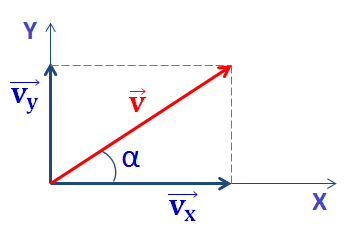
\includegraphics[width=0.55\linewidth]{Figuras/Ch06/decomposicao.png}}
}

\frame{
	\frametitle{Operação com vetores}
	\begin{block}{Vetores unitários}
		Vetor unitário é o que tem o módulo igual a 1. Existem dois vetores unitários que formam a base canônica para o espaço $\mathbb{R}^2$, que são dados por: $\hat{i} = \langle1,0\rangle$ e $\hat{j} = \langle0,1\rangle$
	\end{block}
}

\frame{
	\frametitle{Operação com vetores}
	\begin{block}{Vetores unitários}
		Para fazer cálculos de vetores em apenas um dos planos em que ele se apresenta, pode-se decompor este vetor em vetores unitários em cada um dos planos apresentados. \\
		$$\vec{S} = 3\hat{i} + 4\hat{j}$$
	\end{block}

	\vspace{0.2cm}

	\setmyunit{1.5cm}
	
	\centering
	\begin{tikzpicture}[scale=0.5]
		\draw[-Latex] (0,0) -- node[below] {$ 3\hat{i} $} (3,0);
		\draw[-Latex] (0,0) -- node[left] {$ 4\hat{j} $} (0,4);
		
		\draw[-Latex,red] (0,0) -- node[above] {$ \vec{S} $} (3,4) coordinate (s);
		
		\draw[dashed] (0,4) -- (s) (3,0) -- (s);
	\end{tikzpicture}
	
%	\centerline{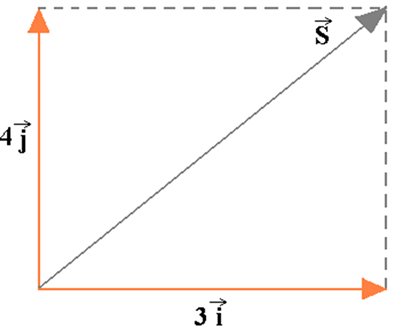
\includegraphics[width=0.4\linewidth]{Figuras/Ch06/unitario.jpg}}
}

\section*{Exercícios}

\frame{
	\frametitle{Exercícios}
	\begin{block}{}

		01. O campo elétrico criado por uma carga pontual, no vácuo, tem intensidade igual a \SI[scientific-notation=true]{9e-1}{\newton\per\coulomb}. Calcule a que distância $d$ se refere o valor desse campo, sendo $Q = \SI{-4}{\pico\coulomb} $.

		\vspace{0.3cm}

		02. (Mackenzie-SP) Determine a intensidade do campo elétrico, num ponto situado a \SI{3.0}{\milli\meter} de uma carga elétrica puntiforme $Q =\SI{2.7}{\micro\coulomb}$ no vácuo.

		\vspace{0.3cm}

		03. Qual é a medida do lado oposto ao ângulo de $\ang{30}$, em um triângulo, sabendo que os outros dois lados medem $2$ e $\sqrt{3}$?
	\end{block}
}


\section*{Referências}

\frame{
	\frametitle{Referências e Exercícios Complementares}
	\begin{itemize}
		\item Física, Ciência e Tecnologia – Vol 3. PENTEADO, Paulo César M; TORRES, Carlos Magno A. Ed. Moderna (2006)
	\end{itemize}
	%\centering{\alert{Página 36 - \textbf{1.6.1 até 1.6.5, 1.6.17 até 1.6.19}}} \\
	%https://www.youtube.com/watch?v=IUgS7Uw-qBI
	\centering{\alert{Lista de exercícios 06}}
}